
 
% ========== Chapter 4
 
\chapter{Alpha Backgrounds in the \MJ\ \DEM\ }\label{ch:MJ_rates}

\section{Introduction}
The \MJ\ \DEM\ has been taking data with its low-background cryostats since June 2015. Using the open data, we can estimate the background rate of alpha decays in the system and attempt to speak to their source. We can evaluate the effectiveness of the DCR pulse-shape discriminator in reducing the background rates, both in the \nonubb\ ROI and at energies over 2.7\,MeV, where we expect alpha particle backgrounds to dominate the spectrum. 

In particular, we focus on the background rates in the enriched detectors, which were produced by ORTEC. These detectors have similar geometries to the PONaMA-1 detector studied with the TUBE scanner (see Chp.~\ref{TUBE_setup} and ~\ref{TUBE_results}); we expect them to respond similarly to the DCR analysis, with the pulse-shape parameter efficiently identifying passivated-surface alpha events occurring on over 97\% of the surface. These detectors also dominate our sensitivity to \nonubb , given their 86\% $^{76}$Ge abundance. 

In the natural-abundance BEGe-type detectors, the background reduction effect of the DCR analysis is expected to be far less than those of a (still-to-be-implemented) near-point-contact event cut, such as an upper limit on the accepted A/E values or a lower limit on the accepted rise times. See Sec.~\ref{sec:ae_completementarity} for further discussion. 

\section{DCR Cut Background Reduction}
The background rates with and without the DCR cut applied to the data were evaluated in Data Sets 0-4. The Data Sets are summarized in Table~\ref{tab:DS_summary}. The exposures listed here do not exactly match those given in the \MJ\ run selection and data cleaning technical document \cite{MJ_runSel}; several detectors in each official data set were disregarded due to incomplete analysis at the time of writing. The runs used (and the criteria used to select runs) are exactly those in \cite{MJ_runSel}. The rates are evaluated separately in each data set, so they may be compared across the two modules and, in Module 1, studied over time. 

\begin{table}[]
\centering
\begin{tabular}{r p{1.5in} l l l p{2in}}
DS & Dates & Modules & \begin{tabular}[c] {@{}l@{}}Exposure\\(kg days)\end{tabular} & \begin{tabular}[c] {@{}l@{}}Enr. Exposure\\(kg days)\end{tabular}& Notes \\
\hline
0 & 6/26 - 10/7/15 & 1 & 509.428 & 324.220 & No inner shield \\
1 & 12/31/15 - 5/24/16 & 1 & 692.845 & 626.779 & \\
2 & 5/24 - 7/14/16 & 1 & 114.368 & 103.520 & Multi-sampling enabled \\
3 & 8/25 - 9/27/16 & 1 & 425.78 & 342.571 & \\
4 & 8/25 - 9/27/16 & 2 & 223.282 & 93.615 & \\
\end{tabular}
\caption{A summary of open data used from the \MJ\ \DEM\ data sets. }
\label{tab:DS_summary} 
\end{table}

\begin{figure}[t]
 \centering
  \begin{subfigure}[]{\textwidth}
  \centering
 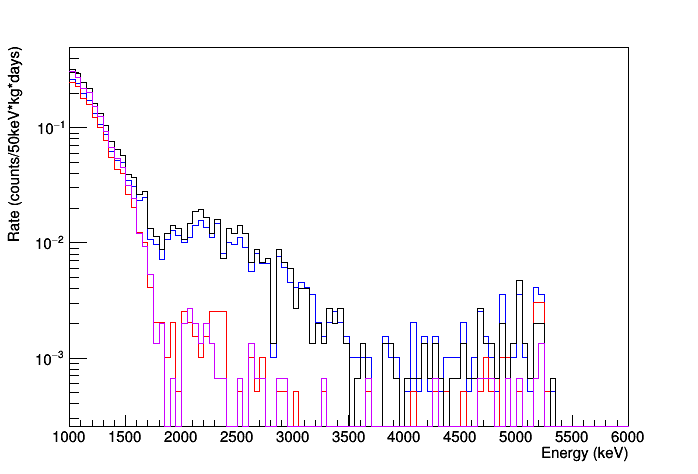
\includegraphics[height=3in]{/Users/jgruszko/Documents/Thesis/Plots/Ch4/sumSpec_all.png}
\end{subfigure}
 % ~
%  \begin{subfigure}[]{\textwidth}
 %  \centering
% 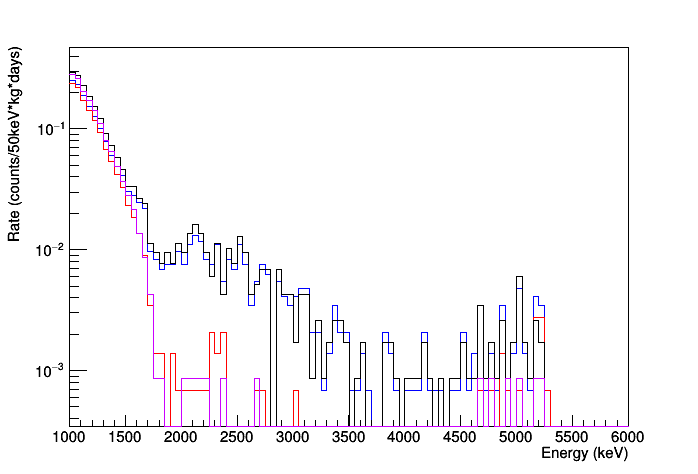
\includegraphics[height=.3\textheight]{/Users/jgruszko/Documents/Thesis/Plots/Ch4/sumSpec_no0.png}
% \end{subfigure}
%\caption[Background rates in \MJ\ data sets 0-4]{Sum spectra of data sets 0-4 {\it (top)} and 1-4 {\it (bottom)}. The blue and red lines give the spectra in all detectors with and without the DCR cut, respectively, and the black and violet lines give the same in only the enriched detectors.}
\caption[The high-energy spectrum in \MJ\ data sets 0-4]{Sum spectrum of data sets 0-4. The blue and red lines give the spectra in all detectors with and without the DCR cut, respectively, and the black and violet lines give the same in only the enriched detectors.}
\label{fig:sumSpec}
\end{figure}


From the summed high-energy spectrum (see Fig.~\ref{fig:sumSpec}), we observe a peak near 5.3\,MeV, the full energy of the alpha decay of $^{210}$Po. This indicates that there is a significant background contribution from the $^{226}$Ra decay chain, though the question of whether the decay chain is in equilibrium remains. $^{210}$Po has a half-life of 138 days, several times shorter than the accumulated run time of the \DEM ; if the decay is unsupported by the long-lived (22 years) $^{210}$Pb isotope, we will observe a falling alpha event rate over the course of these data sets. 

Measurements with the TUBE scanner allow us to conclude that in the enriched detectors, the peak near 5.3\,MeV is due to alpha particles incident on the point-contact itself, since little energy is being lost to charge-trapping in these events. The peak is broader and reaches higher energies than we would expect from the measurement of PONaMa-1, but this is likely due to detector-to-detector variation of the point contact dead layer thickness. 

To evaluate the rate of alpha background events and the effectiveness of the DCR cut, it is appropriate to study three energy regions. At energies between 2.7 and 4.5\,MeV, we expect the dominant background contribution to be alpha particles incident on the passivated surface (or, for BEGe detectors, in the ditch region). The DCR parameter should identify these events as alpha background events with high efficiency, particularly in the enriched detectors. 

We take the energy region from 4.5 to 5.5\,MeV as a generous estimate of the energy range in which alphas incident on the point contact may appear. The DCR parameter is expected to be insensitive to these events.  The use of this large energy window, however, may lead to a contribution from the highest-energy passivated surface events, which the DCR parameter should identify as alpha background events. 

The combined energy window of 2.7 to 5.5\,MeV is used to study the level of $^{210}$Po contamination, the alpha rate over time, and the variation in alpha backgrounds from detector to detector. 

Finally, we also study the energy window used to determine the background in the \nonubb\ region-of-interest, a disjoint 350\,keV window around the \nonubb\ Q-value (2039\,keV) that excises expected gamma background peak regions. The event energies included in this analysis are those from 1950 to 2350\,keV, with the exception of the regions from 2094 to 2127 and 2195 to 2212\,keV. In this region, we expect the source of the background events to be a mixture of gamma Compton continuum events and passivated surface alpha events. Data Set 0, in particular, is expected to have a higher rate of gamma background events in this region, since the inner copper shield and additional cross-arm shielding were not yet in place during these runs.

Given the TUBE scan results, we expect the alpha events in this energy window to originate from a mixture of small radius and large incidence angle events. High incidence angle events are expected to remain at the DCR parameter values that are characteristic of their incidence radii, and will therefore be identified effectively. For the small radius events, the DCR analysis begins to lose power in identifying alpha events at these energies, due to the falling hole-fraction contribution to the signal. These remaining alpha events are expected to be identifiable with high efficiency by a pulse shape discriminator that identifies near-point-contact events, like the high-A/E analysis used in the TUBE analysis. 

\begin{table}[]
\centering
\begin{tabular}{l p{1in} l l l l }
DS & Energy Range & \begin{tabular}[c] {@{}l@{}}Rate\\ (\cpKkgd) \end{tabular} & \begin{tabular}[c] {@{}l@{}}Rate\\after DCR\\ (\cpKkgd)\end{tabular} & \begin{tabular}[c] {@{}l@{}}Enr. Rate\\(\cpKkgd)\end{tabular} & \begin{tabular}[c] {@{}l@{}}Enr. Rate\\after DCR \\(\cpKkgd)\end{tabular} \\
\hline
\hline
0 &  $2.7-4.5$\,MeV &         4.0e-5$^{+6.6e-6}_{-6.6e-6}$ &         5.5e-6$^{+5.4e-6}_{-3.4e-6}$ &         2.9e-5$^{+1.4e-5}_{-1.0e-5}$ &         5.1e-6$^{+7.6e-6}_{-3.2e-6}$  \\
  &  $4.5-5.5$\,MeV &         1.8e-5$^{+1.2e-5}_{-9.1e-6}$ &         1.4e-5$^{+1.1e-5}_{-6.7e-6}$ &         3.1e-6$^{+1.0e-5}_{-2.7e-6}$ &         3.1e-6$^{+1.0e-5}_{-2.7e-6}$  \\
  &             ROI &         4.5e-4$^{+5.0e-5}_{-5.0e-5}$ &         5.6e-5$^{+3.6e-5}_{-2.5e-5}$ &         6.3e-4$^{+7.4e-5}_{-7.4e-5}$ &         5.3e-5$^{+4.8e-5}_{-3.3e-5}$  \\
\hline
1 &  $2.7-4.5$\,MeV &         3.4e-5$^{+5.3e-6}_{-5.3e-6}$ &         0$^{+2.0e-6}_{-0}$ &         3.6e-5$^{+5.7e-6}_{-5.7e-6}$ &         0$^{+2.2e-6}_{-0}$  \\
  &  $4.5-5.5$\,MeV &         4.3e-5$^{+1.5e-5}_{-1.2e-5}$ &         1.6e-5$^{+9.8e-6}_{-7.3e-6}$ &         3.7e-5$^{+1.4e-5}_{-1.1e-5}$ &         8.0e-6$^{+8.0e-6}_{-5.0e-6}$  \\
  &             ROI &         2.0e-4$^{+2.9e-5}_{-2.9e-5}$ &         2.5e-5$^{+2.3e-5}_{-1.6e-5}$ &         2.1e-4$^{+3.1e-5}_{-3.1e-5}$ &         1.4e-5$^{+2.0e-5}_{-8.6e-6}$  \\
\hline
2 &  $2.7-4.5$\,MeV &         3.4e-5$^{+2.7e-5}_{-1.7e-5}$ &         0$^{+1.2e-5}_{-0}$ &         3.8e-5$^{+3.0e-5}_{-1.8e-5}$ &         0$^{+1.3e-5}_{-0}$  \\ 
  &  $4.5-5.5$\,MeV &         2.6e-5$^{+3.9e-5}_{-1.7e-5}$ &         8.7e-6$^{+2.9e-5}_{-7.8e-6}$ &         1.9e-5$^{+3.8e-5}_{-1.4e-5}$ &         0$^{+2.4e-5}_{-0}$  \\
  &             ROI &         1.7e-4$^{+1.4e-4}_{-8.6e-5}$ &         0$^{+6.1e-5}_{-0}$ &         1.7e-4$^{+1.5e-4}_{-1.0e-4}$ &         0$^{+6.7e-5}_{-0}$  \\
\hline
3 &  $2.7-4.5$\,MeV &         4.8e-5$^{+7.9e-6}_{-7.9e-6}$ &         1.3e-6$^{+4.4e-6}_{-1.2e-6}$ &         3.7e-5$^{+1.5e-5}_{-1.2e-5}$ &         0$^{+4.0e-6}_{-0}$  \\
  &  $4.5-5.5$\,MeV &         2.6e-5$^{+1.6e-5}_{-1.2e-5}$ &         7.0e-6$^{+1.0e-5}_{-4.5e-6}$ &         2.3e-5$^{+1.8e-5}_{-1.2e-5}$ &         2.9e-6$^{+9.8e-6}_{-2.6e-6}$  \\
  &             ROI &         1.7e-4$^{+6.4e-5}_{-5.0e-5}$ &         1.3e-5$^{+2.6e-5}_{-9.8e-6}$ &         1.8e-4$^{+7.5e-5}_{-5.8e-5}$ &         0$^{+2.0e-5}_{-0}$  \\
\hline
4 &  $2.7-4.5$\,MeV &         3.5e-5$^{+1.9e-5}_{-1.4e-5}$ &         2.5e-6$^{+8.4e-6}_{-2.2e-6}$ &         4.2e-5$^{+3.3e-5}_{-2.0e-5}$ &         0$^{+1.4e-5}_{-0}$  \\
  &  $4.5-5.5$\,MeV &         4.5e-6$^{+1.5e-5}_{-4.0e-6}$ &         0$^{+1.1e-5}_{-0}$ &         0$^{+2.6e-5}_{-0}$ &         0$^{+2.6e-5}_{-0}$  \\
  &             ROI &         2.8e-4$^{+1.2e-4}_{-8.9e-5}$ &         1.3e-5$^{+4.3e-5}_{-1.1e-5}$ &         6.4e-4$^{+2.7e-4}_{-2.1e-4} $&         0$^{+7.4e-5}_{-0}$  \\
\hline
\hline
0-4 &  $2.7-4.5$\,MeV &         4.4e-5$^{+3.5e-6}_{-3.5e-6}$   &         2.8e-6$^{+1.8e-6}_{-1.3e-6}$  &          4.1e-5$^{+ 3.9e-6}_{-3.9e-6}$ &         2.2e-6$^{2.0e-6}_{-1.4e-6}$ \\
  &  $4.5-5.5$\,MeV &         2.8e-5$^{+3.8e-6}_{-3.8e-6}$   &         1.2e-5$^{+4.6e-6}_{-3.7e-6}$  &          2.4e-5$^{+ 7.4e-6}_{-6.1e-6}$ &         5.4e-6$^{4.0e-6}_{-2.7e-6}$ \\
  &             ROI &         2.7e-4$^{+2.0e-5}_{-2.0e-5}$   &         3.6e-5$^{+1.4e-5}_{-1.1e-5}$  &          3.1e-4$^{+ 2.5e-5}_{-2.5e-5}$ &         2.9e-5$^{1.4e-5}_{-1.1e-5}$ \\
\hline
1-4 &  $2.7-4.5$\,MeV &         3.9e-5$^{+3.8e-6}_{-3.8e-6}$   &         7.6e-7$^{+1.5e-6}_{-5.6e-7}$  &          3.7e-5$^{+ 4.2e-6}_{-4.2e-6}$ &         0$^{1.2e-6}_{-0}$ \\
 &  $4.5-5.5$\,MeV &         3.1e-5$^{+4.6e-6}_{-4.6e-6}$   &         1.0e-5$^{+5.2e-6}_{-3.8e-6}$  &          2.8e-5$^{+ 9.0e-6}_{-7.7e-6}$ &         5.1e-6$^{4.7e-6}_{-3.2e-6}$ \\
 &             ROI &         2.0e-4$^{+2.0e-5}_{-2.0e-5}$   &         1.8e-5$^{+1.2e-5}_{-9.1e-6}$  &          2.3e-4$^{+ 2.4e-5}_{-2.4e-5}$ &         7.3e-6$^{1.1e-5}_{-4.6e-6}$ \\                                                                                                                  
\end{tabular}
\caption[Background rate results in \MJ\ \DEM\ data sets 0-4] {Background rate results in \MJ\ \DEM\ data sets 0-4, with and without the DCR cut applied to the data.}
\label{tab:bkg_rates} 
\end{table}

In addition to the appropriate energy, channel, and run selection, events must pass muon veto, data cleaning, granularity, and single-site (A vs. E) event cuts, and must not occur during the LN-fill veto period. Rates are presented for the sum of all detectors and for only enriched (ORTEC-type) detectors, both with and without the 90\% bulk-acceptance DCR cut applied to the events. For results, see Table~\ref{tab:bkg_rates} and Fig.~\ref{fig:rate_plots}.

\begin{figure}[]
 \centering
  \begin{subfigure}[]{\textwidth}
  \centering
 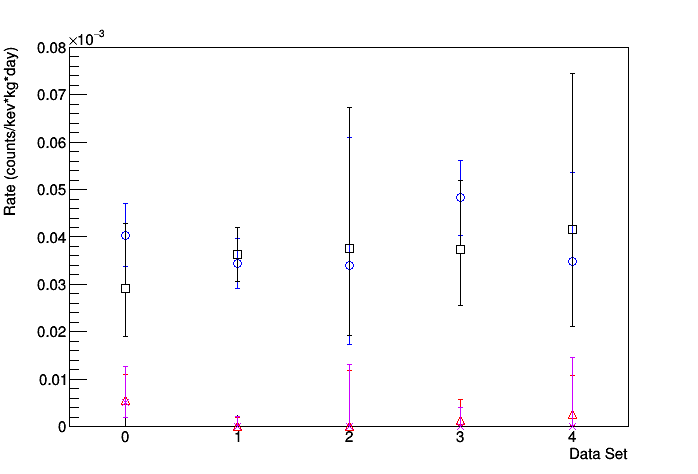
\includegraphics[height=.3\textheight]{/Users/jgruszko/Documents/Thesis/Plots/Ch4/DSrates_2700to4500keV.png}
 \label{fig:pass_rate}
\end{subfigure}
  ~
  \begin{subfigure}[]{\textwidth}
   \centering
 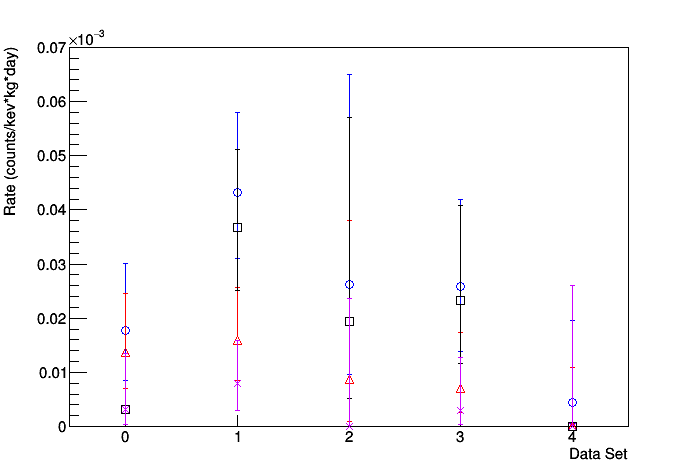
\includegraphics[height=.3\textheight]{/Users/jgruszko/Documents/Thesis/Plots/Ch4/DSrates_4500to5500keV.png}
 \label{fig:peak_rate}
 \end{subfigure}
 ~
   \begin{subfigure}[]{\textwidth}
   \centering
 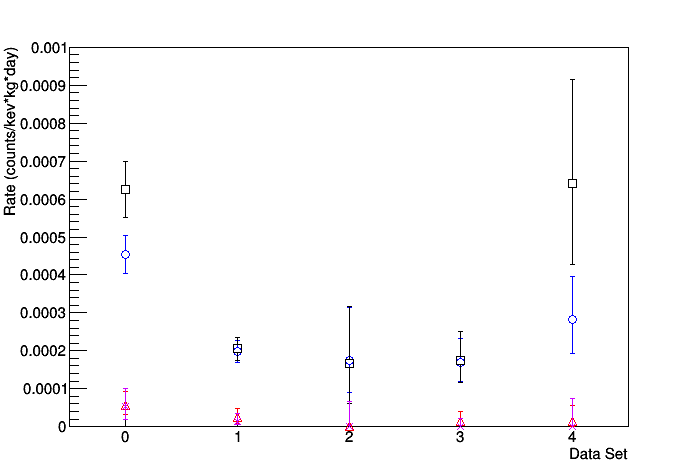
\includegraphics[height=.3\textheight]{/Users/jgruszko/Documents/Thesis/Plots/Ch4/DSrates_ROI.png}
 \label{fig:ROI_rate}
 \end{subfigure}
\caption[Background rates in \MJ\ data sets 0-4]{Rates in the 2.7 to 4.5\,MeV {\it (top)}, 4.5 to 5.5\,MeV  {\it (middle)}, and ROI {\it (bottom)} energy windows. Blue circles and and red triangles represent the rates in all detectors with and without the DCR cut, respectively, and black squares and violet crosses give the same in only the enriched detectors.}
\label{fig:rate_plots}
\end{figure}

From these results, there is little indication of a change in the alpha event rate over the course of the data sets. As expected, the DCR analysis reduces the background rate quite effectively in the passivated surface and ROI energy windows, but has little effect in the energy region of the full-energy $^{210}$Po events. In the enriched detectors, no events remain in the 2.7 to 4.5\,MeV window following the DCR cut in any of data sets 1 through 4.

\section{Rate Analysis}
\begin{figure}[t]
  \centering
 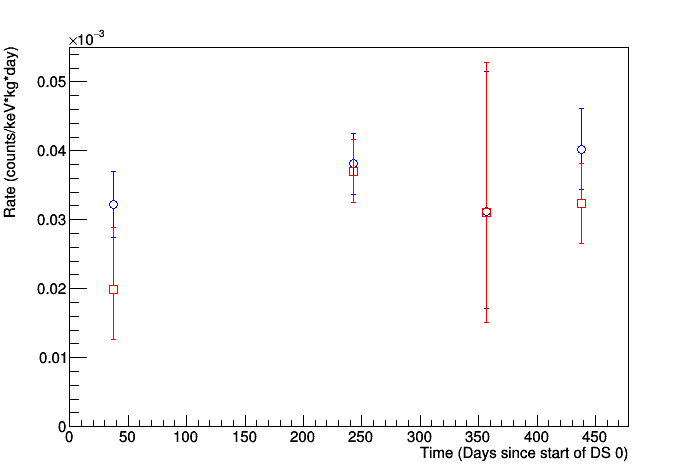
\includegraphics[height=3in]{/Users/jgruszko/Documents/Thesis/Plots/Ch4/rates_byDS.png}
\caption[M1 alpha background rates in \MJ\ data sets 0-3, as a function of time]{M1 alpha background rates in the 2.7 to 5.5\,MeV energy window of each data set, given as a function of time. Blue circles indicate the rates in all detectors, and red squares are the rates in only enriched detectors. The DCR cut is not applied, but single-site, muon, granularity, and data cleaning cuts are applied to the data.}
\label{fig:rates_byDS}
\end{figure}

To evaluate the rate over time, we use the energy window from 2.7 to 5.5\,MeV. Given the low alpha event rates, we average over each data set. As the date of the integrated rate in each data set, we use the exponentially-weighted average date:
$$\overline{t} = \frac{\sum_{i=0}^{n}te^{\frac{-(t_i+\Delta t/2-t_0)}{\tau}}\Delta t }{\sum_{i=0}^{n}e^{\frac{-(t_i+\Delta t/2-t_0)}{\tau}}\Delta t} $$
where $\tau = t_{1/2}/\ln(2) = 199.7$\,days is the decay constant of $^{210}$Po and the sums are taken over each of the $n$ runs of the data set. $t_i$ and $\Delta t$ are the start times of each run, and $t_0$ is the start time of the data set, taken as the number of days since the beginning of DS0 data-taking. 

As seen in Fig.~\ref{fig:rates_byDS}, there is no hint of decay in the alpha background rates over time. All of the data set rates are in agreement except for the rate in the DS 0 enriched detectors, which is in tension with the equivalent rate in DS1 and in slight tension with that from DS3. In spite of the high statistical errors associated with the rates, the decay would be clearly detectable if the entirety of the alpha background contribution were due to unsupported $^{210}$Po decay; the expected rate after 350 days is less than 20\% of the starting rate, well outside the statistical errors of the rates. Therefore we must conclude that at least the majority of the alpha backgrounds are supported by $^{210}$Pb decay. 

The total observed $^{210}$Po activity in the 2.7 to 5.5\,MeV window is 13.1$\pm$1.0\,$\mu$Bq, and the total in this energy range in the enriched detectors is 8.8$\pm$0.8$\mu$Bq. These values should be considered to be lower limits on the $^{210}$Po activity, since an unknown fraction of events occur at energies below 2.7\,MeV. 

\section{Detector-by-detector Backgrounds}

\begin{figure}[t]
  \centering
 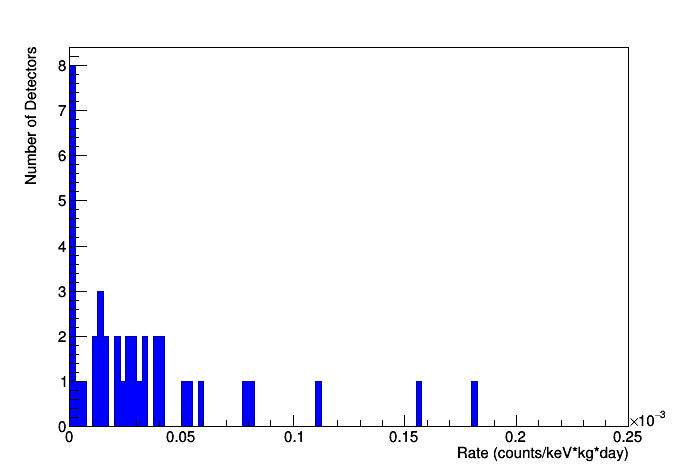
\includegraphics[height=3in]{/Users/jgruszko/Documents/Thesis/Plots/Ch4/rateDist_all.png}
\caption[The distribution of alpha background rates]{The distribution of the number of detectors with a given alpha background rate. 7 of the 8 detectors with rates over 5E-5\cpKkgd\ appear on the list in Table~\ref{tab:hotDets}. The remaining detector is B8463, a BEGe-type (natural) detector with a high uncertainty in its rate due to its small exposure.}
\label{fig:rateDist}
\end{figure}

The \MJ\ Collaboration is very interested in discovering the source of the alpha background contamination, so that it may, if possible, be removed. To this end, it is also of interest to examine the alpha background rates observed on a detector-by-detector basis, to find whether some detectors are particularly contaminated. Even if the alpha background cannot be eliminated in during the life of the \MJ\ \DEM , understanding its source will allow future low-background HPGe-based experiments to limit this problematic background. 

Again, we integrate the single-site, non-muon events with energies between 2.7 and 5.5\,MeV following granularity, LN fill, and data cleaning cuts. The error associated with each detector varies, as their both their masses and operating times vary. 

\begin{table}[t]
\centering
\begin{tabular}{p{1in} l l l l}
Det. & Type & All & Enr. & Rate \\
\hline
P42538B  & Enr. & \checkmark & \checkmark &    1.6e-04$^{+4.4e-05}_{-3.8e-05}$ \\ 
P42661C  & Enr. &            & \checkmark &    1.1e-04$^{+4.3e-05}_{-3.3e-05}$ \\
  B8455  & Nat. & \checkmark & \checkmark &    1.8e-04$^{+7.5e-05}_{-5.8e-05}$ \\
P42853B  & Enr. & \checkmark & \checkmark &    5.8e-05$^{+6.7e-05}_{-3.7e-05}$ \\
  B8466  & Nat. & \checkmark & \checkmark &    8.0e-05$^{+1.2e-04}_{-5.0e-05}$ \\
  B8481  & Nat. & \checkmark & \checkmark &    5.2e-05$^{+1.0e-04}_{-3.8e-05}$ \\
  B8594  & Nat. & \checkmark & \checkmark &    8.1e-05$^{+1.2e-04}_{-5.1e-05}$ \\
\end{tabular}
\caption[The list of high-alpha activity detectors]{7 detectors were found to have alpha rates inconsistent with the average rates. A checked box in the ``All" column indicates that the rate is inconsistent with the average rate across all detectors, and a checked box in the ``Enr." column indicates that it it inconsistent with the (lower) average rate in the enriched detectors.}
\label{tab:hotDets}
\end{table}

The integral rates for each of the detectors (including data sets 0-4) can be seen in Fig.~\ref{fig:rates_byDet}. In addition to the Poisson errors for these rates, we give the Feldman-Cousins \cite{FeldmanCousins}upper and lower bounds for an expected background of 0. Since the rates are very close to 0, the FC procedure allows us to present rates that transition smoothly to upper limits when a rate of 0 is measured, without under-coverage.  

The average rate, when taken among all the detectors, is 3.4e-05$\pm$4.0e-06 \cpKkgd . When taken among only the enriched detectors, it is 2.67e-05$\pm$4.4e-06  \cpKkgd. The difference in these averages does not necessarily imply that the $^{210}$Po average activity levels differs between the enriched and natural-abundance detectors, since only the alpha spectrum above 2.7\,MeV is used to find this rate. If the BEGe-type detector design leads to fewer highly energy-degraded events (with energies less than 2.7\,MeV) than the ORTEC geometry, these rates would be brought into closer agreement. 

Using these two averages, we find the detectors that are inconsistent with the average rate, as defined by their FC limits (i.e. their lower FC bound is above one or both of the averages). These high-alpha rate detectors are given in Table~\ref{tab:hotDets}. These detectors also appear as outliers in the distribution of detector alpha rates, seen in Fig.~\ref{fig:rateDist}. 

\begin{sidewaysfigure}[]
  \centering
 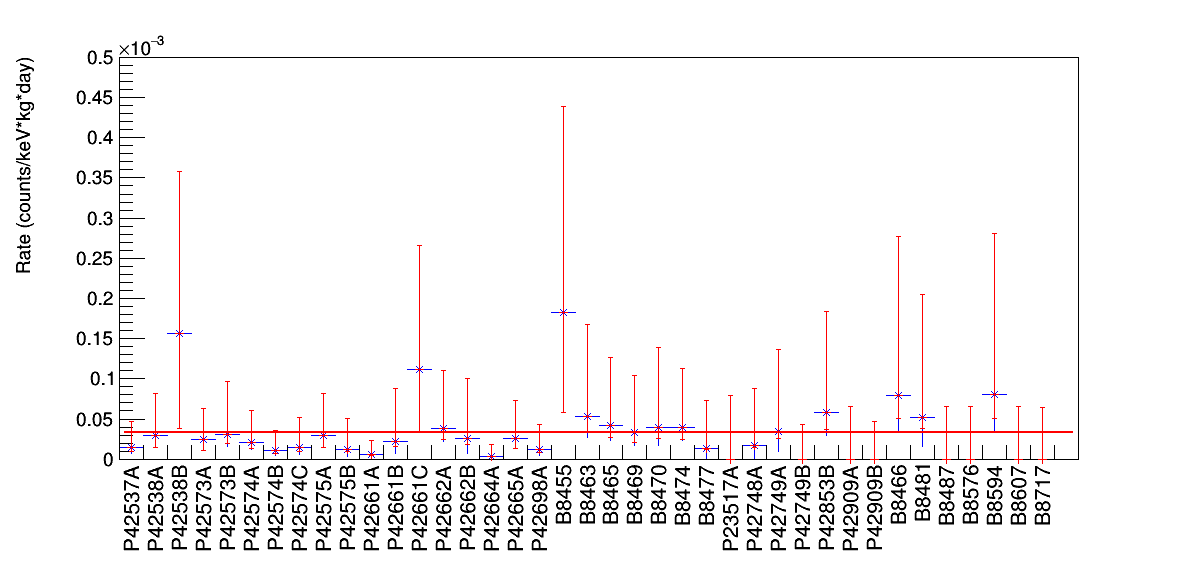
\includegraphics[width = 1.0\textwidth]{/Users/jgruszko/Documents/Thesis/Plots/Ch4/rates_byDet_all_zoomOut.png}
\caption[Alpha background rates in all detectors]{Rates in the 2.7 to 5.5\,MeV energy window for each detector. Blue points indicate the Poisson error bounds, and red points indicate the Feldman-Cousins intervals. The average for all detectors is indicated by the red line.}
\label{fig:rates_byDet}
\end{sidewaysfigure}

The potential origins of the elevated alpha background rates in these detectors are currently being investigated. The \MJ\ Collaboration has carefully tracked the manufacturing, cleaning, storage, and assembly history of all the detectors and parts \cite{PTDB}, and is now studying these records to find the shared elements in these detectors' histories. 

\section{DCR Effect on \nonubb\ Sensitivity}
The half-life sensitivity to \nonubb\ is given by:
$$ T^{0\nu}_{1/2} > \ln 2 \frac{N_a t \varepsilon }{\langle \mathrm{UL}(B(t))\rangle}, $$
where $N_a$  is the number $^{76}$Ge atoms, $t$ is the live time, $\varepsilon$ is the efficiency, and $B(mt)$ is the predicted number of background events after the integrated exposure $mt$. $\langle$UL$(B)\rangle$ denotes the average upper limit an ensemble of identical experiments would place in the absence of a signal given $B$ background counts \cite{Detwiler_sensitivity}. In the nearly background-free regime, the Feldman-Cousins method \cite{FeldmanCousins} provides an appropriate means to calculate this value for a given observed background level. At high background levels, $\langle$UL$(B)\rangle = \sqrt B$. 

To calculate the expected background level in the \nonubb\ ROI, we assume that the background spectrum is flat, except for the excised gamma peak regions, in the 400\,keV window around the 2039\,keV Q-value. Since the enriched detectors drive the \MJ\ \DEM 's sensitivity, we are most interested in the decrease in the backgrounds due to the DCR cut in these detectors. We do not consider Data Set 0 in this analysis, since it was taken with incomplete shielding and is known to have higher gamma backgrounds than the final configuration of the \DEM. 

In data sets 1 through 4, the use of the 90\% bulk-acceptance DCR cut reduces the enriched detector event rate in the \nonubb\ ROI background-estimate window from from 93 counts to 3 counts, a factor of 31 reduction. As seen in Table~\ref{tab:bkg_rates}, this corresponds to a reduction in the rate from 2.3e-4$^{+ 2.4e-5}_{-2.4e-5}$\,\cpKkgd\ to 7.3e-6$^{1.1e-5}_{-4.6e-6}$\,\cpKkgd . 

To calculate $\langle$UL$(B)\rangle$ we must first find $B$, the expected number of background events in the ROI in time $t$. For the purposes of this calculation, we take $mt$ to be the accumulated enriched exposure of Data Sets 1-4, 1166.505\,kg days. The background index given above must be multiplied by the width of the ROI in keV. Given small changes in the detector resolution between data sets, the optimal width of the ROI has changed slightly over the course of the experiment; we take it to be the exposure-weighted average of the ROI widths in each of the data sets, 2.99\,keV. 

Multiplying by these values, we find an expected number of background events of 0.80$^{0.08}_{0.08}$ without the DCR cut, and 25E-3$^{39E-3}_{16E-3}$ with the DCR cut.  Therefore the average upper limit in the absence of a signal, $\langle$UL$(B)\rangle$, is 1.72 without the DCR cut, or 2.41 with it. Given that the 90\% bulk acceptance of the DCR cut gives $\varepsilon \prime = 0.9\varepsilon$, the sensitivity without the DCR cut is:
$$T^{0\nu}_{1/2} >  \ln 2 \frac{N_a t \varepsilon }{1.72},$$
and with the DCR cut it is:
$$T^{0\nu \prime}_{1/2}  >  \ln 2 \frac{N_a t 0.9\varepsilon }{2.41} = 0.64\,T^{0\nu}_{1/2}. $$
We conclude the the application of the DCR cut improves the \nonubb\ sensitivity of the \MJ\ \DEM\ by a factor of 1.6. In other words, the experiment is sensitive to decay lifetimes about two-thirds as long as the lifetimes it would be sensitive to without the DCR cut in place. 

\section{Identifying the Source of Alpha Events in the \MJ\ \DEM\ }
\subsection{Projected Alpha Energy Spectrum}\label{ssec:alpha_model}
To create a realistic alpha energy spectrum, the radial dependence of the energy found with the TUBE scan, derived in Sec.~\ref{sssec:spec_fit} must be integrated with respect to position for a given model of the alpha contamination, and corrected for the alpha particle incidence angle energy-dependence. Below, we derive the expected energy spectra for two potential models of contamination: a uniform-distribution model, and a point-source contamination model.  

Also needed is the fraction describing the relative deadness of the point-contact region, compared to the passivated surface. In the TUBE measurements, the alpha rate at unobscured scanning positions incident on the passivated surface, derived in Sec.~\ref{ssec:alpha_rate} is constant, with an average of 64.6\,events/hr. The peak in the data sets with the source fully incident on the point-contact, on the other hand, shows a substantially reduced event rate, likely due to the thicker dead-layer in this region. Combining all data sets taken with the source incident at $r=-0.75$\,mm, we find an average rate of $3.9\pm.3$\,events/hr. The full-energy peak fraction $f_{pk}$ is then 0.06. 

This should be considered a lower bound for the detectors in the \DEM , since the point-contact is partially obscured by the contact pin in the TUBE measurements, reducing the event rate. Depending on the source of alpha background events, the obstruction of the point-contact region by the contact-pin in a low-background experiment could similarly reduce the rate, or leave it unchanged (if the contamination lay between the point contact and the detector surface). The contact pin in the \MJ\ detector mount is slightly smaller than that used in TUBE (get dimensions, if possible), so $f_{pk}$ would be correspondingly larger, even if the alpha source were similarly obstructed by the pin.

\subsubsection{Uniform-distribution Model}
The uniform-distribution model of alpha contamination assumes a constant distribution $\sigma$ of alpha-emitters across the entire detector surface, including the point-contact region. This model mimics the distribution that would be expected if, for instance, the detector were exposed to $^{226}$Rn during fabrication or construction, leading to a uniform distribution of $^{210}$Po decays on the surface. This model would also be appropriate for the case of a uniform distribution of alpha emitters on the surfaces of copper parts, since the crystal mounting plate, the copper part that is closest to the passivated surface in the \MJ\ detector mount design, is roughly equidistant from all points on the passivated surface and point contact. 

Beginning with the contamination model:
$$n(r, \phi) = \sigma r \mathrm{d}r \mathrm{d}\phi, $$
where $\phi$ is the azimuthal angle, we split it into point-contact and passivated surface terms. The point-contact component is integrated over the entire point contact region to derive a rate for this contribution, since the energy is independent of radius in this region. 

The passivated surface term has a one-to-one correspondence of energy to radius, so one can integrate in the azimuthal angle dimension and transform from the radius to the energy variable to give a rate in terms of energy, i.e., an energy spectrum:
$$n(E)\mathrm{d}E =  f_{pk}\delta(E-E_{pk})\sigma \int_{0}^{r_p} \int_{0}^{2\pi}r{d}r \mathrm{d}\phi \\
+ \sigma \int_{0}^{2\pi}r(E)\mathrm{d}r(E) \mathrm{d}\phi 
$$
Where $f_{pk} = .06$ is the deadness fraction of the point contact derived above, $E_{pk}= 5323$\,keV is the average energy of the point-contact alpha events, and $r_p = 1.6$\,mm is the point contact radius. Substituting the radial dependence on energy (found in Sec~\ref{sssec:spec_fit}) and the corresponding Jacobean in the second term:
\begin{equation}
\begin{split}
n(E)\mathrm{d}E = f_{pk}\delta(E-E_{pk})\sigma \int_{0}^{r_p} \int_{0}^{2\pi}r{d}r \mathrm{d}\phi \\
+  \Theta(E_{max}-E)\int_{0}^{2\pi}\sigma(aE^4 + r_p)(4aE^3)\mathrm{d}E \mathrm{d}\phi
\end{split}
\end{equation}
\vspace{1cm}
where $a = 5.50E-14$ is the scaling parameter from the fit and $E_{max} = \sqrt[4]{\frac{r_{max}-r_p}{a}} = 4746\mathrm{keV}$. 
Integrating with respect to $\phi$:
\begin{equation}
\begin{split}
n(E)dE = \pi r_p^2 f_{pk}\sigma\delta(E-E_{pk}) \\
+ 8\pi \sigma a (aE^7 + r_pE^3) \mathrm{d}E.
\end{split}
\end{equation}

Finally, this energy spectrum should be convolved with the spectral peak shape function at each energy. Since the distribution of passivated surface events is very broad compared to the resolution of the energy peaks, this will have little effect on the shape of the passivated surface contribution. The delta function of the point-contact events, on the other hand, will become a Gaussian+low-energy tail peak like those found in the fits of point-contact events. We apply the convolution to only the point-contact events, and set $\sigma$ to 1, to plot the spectrum in Fig.~\ref{fig:spec_shape}.
 
\subsubsection{Point-contact Contamination Model, without Incidence Angle Dependence}\label{sssec:point_model_noAngle}
The other contamination model studied is one in which the alpha events originate in a point source some height $h$ above the center of the p+ contact, and the event rate falls as $\frac{1}{r^2+h^2}$ across the passivated surface of the detector. Possible sources of such a distribution in the \MJ\ \DEM\ would be contamination of the point-contact region of the detector itself, or of the contact pin, tin coating of that pin, or PTFE bushing that holds it in place. 

To avoid a divergence at $r=0$, we assume the contamination on the point-contact itself is uniform, and matches the contamination at the boundary of the point-contact region. 

In this case, the contamination model is:
$$n(r, \phi)=
\begin{cases}
\frac{\sigma}{r_p^2} r(E) \mathrm{d}r \mathrm{d}\phi, r<r_p \\
\frac{\sigma}{r(E)^2+h^2} r(E) \mathrm{d}r \mathrm{d}\phi, r>r_p
\end{cases}
$$

Proceeding as before, the spectral shape is:
\begin{equation}
\begin{split}
n(E)dE &= \pi f_{pk}\sigma\delta(E-E_{pk}) \\
&+ 8\pi \sigma a \frac{(aE^3)(aE^4+r_p)}{(aE^4+r_p)^2+h^2} \mathrm{d}E
\end{split}
\end{equation}
Note that the point-contact contribution is identical as in the uniform contamination model, save for the numerical factor of $1/r_p^2$. Again, we convolve the delta function with the appropriate peak shape and set $\sigma$ to 1 to plot the predicted spectrum, in Fig.~\ref{fig:spec_shape}. 

\begin{figure}[]
 \centering
 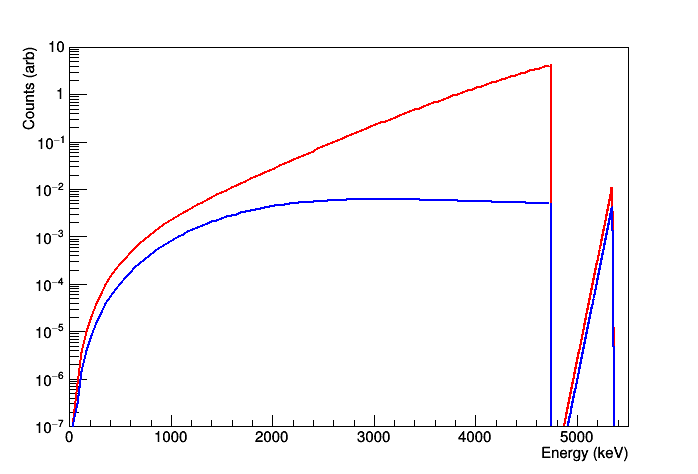
\includegraphics[height=3in]{/Users/jgruszko/Documents/Thesis/Plots/Ch6/spec_shape.png}
 \caption[The predicted energy spectra for the uniform and point-contact contamination models]{The predicted energy spectra for the uniform (in red) and point-contact (in blue) contamination models, without angle-of-incidence correction.} 
 \label{fig:spec_shape}
\end{figure}


\subsubsection{Point-contact Contamination Model, with Incidence Angle Dependence}
The predicted spectral shape derived in Sec.\ref{sssec:point_model_noAngle} does not account for the radial dependence of the alpha particle's incidence angle. Though that would have a minor effect in the uniform contamination model, where most alphas would penetrate normal or nearly normal to the passivated surface, the point-contact contamination model would have a strong radial dependence of incidence angle, with primarily large-incidence-angle scatters occurring at large-radius positions. These events would likely have less energy at a given radius than those measured here, since they would traverse more of the high charge-trapping near-surface region. This would create a large enhancement in the low energy portion of the spectrum, and a corresponding reduction at the high energy portion.

To incorporate the incidence angle energy dependence into the polynomial spectral shape model, we assume that charge-trapping occurs over some constant depth of the region below the passivated surface, and that the amount of energy lost to trapping depends linearly on the path length in this region. Therefore the energy at a given incidence angle $\theta$, where $\theta$ is measured with respect to the horizontal passivated surface, is:
$$ E(r, \theta) = E_0 - \frac{\sin\theta_0}{\sin\theta}(E_0-E(r, \theta_0))$$
where $\theta_0 = 65\degree$ is the incidence angle of the TUBE scan measurements, $E_0$ is the alpha decay energy, and $E(r)$ is the measured spectral shape.

To integrate over the detector surface, we must transform $\theta$ dependence into a dependence on $r$. Given a point-source of alpha particles at height $h$, $\theta = \tan(\frac{h}{r})$. Then the corrected energy $E_f$ is given by:
$$E_f(r)= \frac{\sin\theta_0}{h} \sqrt{h^2+r^2}(E_0-E_i(r, \theta_0)).$$
where $E_i$ is the measured energy in TUBE. 

We can put this in the form of a linear transformation of $E_i$:
\begin{equation}
\begin{split}
E_f(r) &= u(r)E_i+v(r) \\
u(r) &= \frac{\sin\theta_0}{h}\sqrt{h^2+r^2} \\
v(r) &= E_0(1-\frac{\sin\theta_0}{h}\sqrt{h^2+r^2})
\end{split}
\end{equation}
As before, 
$$ r(E_i) = aE_i^4 +r_p. $$
Again, the spectral shape can be found by transforming variables to re-scale the energy axis of the spectrum found in Sec.\ref{sssec:point_model_noAngle}. In this case, the transformation is from the $E_i$ coordinate to the incidence-angle weighted $E_f$. In other words, these two equations are substituted into the spectrum, along with the Jacobean of the transformation from $E_i$ to $E_f$. 
Making the substitution explicit: 
\begin{equation}
\begin{split}
n(E_f)dE_f &= \pi f_{pk}\sigma\delta(E-E_{pk}) \\
&+ 8\pi \sigma a \frac{(E_f(r(E_i))^3)(aE_f(r(E_i))^4+r_p)}{(aE_f(r(E_i))^4+r_p)^2+h^2} \mathrm{d}E_f
\end{split}
\label{eqn:r2_spec}
\end{equation}
where, writing $r$ rather than $r(E_i)$ for the sake of concision:
\begin{equation}
\begin{split}
\mathrm{d}E_f &= E_i\mathrm{d}u(r)+u(r)\mathrm{d}E_i + \mathrm{d}v \\
&= (-r(\frac{\sin\theta_0}{h})(\frac{E_0-E_i}{\sqrt{h^2+r^2}})(4aE_i^3)+\frac{\sin\theta_0}{h}\sqrt{h^2+r^2})\mathrm{d}E_i
\end{split}
\label{eqn:r2_jac}
\end{equation}
For varying heights $h$ of the source, this gives the spectrum pictured in Fig.~\ref{fig:r2_spec_wH}

\begin{figure}[t]
 \centering
 \begin{subfigure}[]{.7\textwidth}
 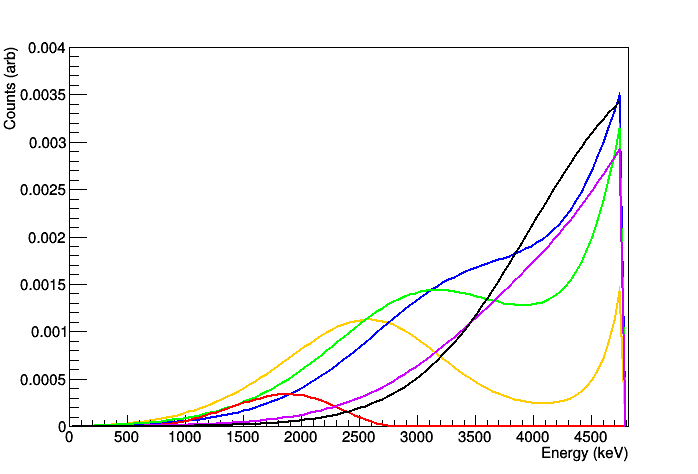
\includegraphics[height=3in]{/Users/jgruszko/Documents/Thesis/Plots/Ch4/varyingH.png}
 \end{subfigure}
  \begin{subfigure}[]{.25\textwidth}
 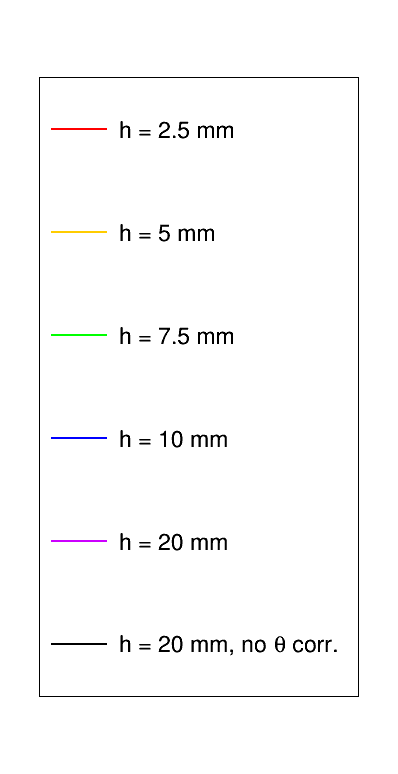
\includegraphics[height=3in]{/Users/jgruszko/Documents/Thesis/Plots/Ch4/r2spec_leg.png}
 \end{subfigure}
 \caption[The predicted energy spectra for the point-contact contamination model, as $h$ varies]{The predicted energy spectra for the point-contact contamination model, as $h$ varies. The black curve does not include the incidence angle correction. The alpha source rate $\sigma$ is set to 1 for all curves.} 
 \label{fig:spec_shape}
\end{figure}

\subsubsection{$^{210}$Po Modifications to the Spectral Model}
The constructed alpha spectra are scaled to the energy of the $^{241}$Am alpha decay. To apply it to the \MJ\ \DEM\ data, we must rescale it to match the energy of the particle emitted by $^{210}$Po, our most significant observed alpha peak. The energy of that decay is 5.304\,MeV, as opposed to $^{241}$Am's most probably decay of 5.485\,MeV. 

Given the charge-trapping model for alpha interactions that we have developed, it is most appropriate to simply rescale the energy in the passivated surface spectral shape function by the ratio of the two energies, so $E_i' = \frac{5.305}{5.485}E_i$.

The point-contact energy function, on the other hand, is best understood as charge loss to a dead layer, which reduces the peak energy by a fixed quantity. This loss is independent of the incident alpha energy, since the energy loss rate $\mathrm(d)E/\mathrm{d}x$ is independent of energy at these alpha energies. Therefore we shift this function by the difference in the energies (180\,keV), rather than applying a scaling factor. 

An important caveat is that this spectral shape has a dependence on the radii of the detector and the point contact. Though PONaMA-1 is a typical detector in these respects, the detectors operating in the \MJ\ \DEM\ vary in both of these dimensions. Similarly, the point-contact dead layers may vary from one detector to another. 

\section{Fitting to the \MJ\ \DEM\ Spectrum}
Comparing the projected alpha spectral models to the high-energy spectra in the \MJ\ \DEM\, we find several things of note. The uniform contamination model is immediately disfavored; its fit to the observed spectrum is far worse than that of the point-contact contamination model. 

Using the spectral shape model given by Eqns.~\ref{eqn:r2_spec} and ~\ref{eqn:r2_jac}, we fit the \MJ\ spectrum in the enriched detectors, with the parameters $\sigma$ and $h$ determined by the fit. All events in data sets 1-4 are used, following data cleaning, LN-fill veto, muon veto, granularity, and A vs. E cuts. The DCR cut is not used, since the goal of this analysis is to pinpoint the source of the alpha events. The energy range used for the fit is from 1900\,keV to $E_{max}$, the endpoint of the PONaMa-1 passivated surface spectrum, scaled to adjust for the $^{210}$Po decay energy, 4611\,keV. The lower energy bound is chosen to avoid a large contribution from \twonubb decay. 

The p+ contact event contribution is not used to fit the spectrum, it is simply drawn with the scaling determined by the passivated surface fit. The background level for the peak is set to the rate at the endpoint of the passivated surface spectrum. 

The alpha activity parameter $\sigma$ fits to a value of 2400$\pm$200\,mm$^{-1}$, and the height $h$ fits to a value of 4.07$\pm$0.06\,mm. The fit is done using the MINUIT log-likelihood fitting algorithm, given the low count rates in the high-energy data.  The predicted spectrum fit the data quite well, as seen in Fig.~\ref{fig:r2spec_orig}; it actually overfits the data, giving a $\chi^2/N_{DF}$ of 0.52. This is because the Gaussian error assumption of the $\chi$ estimator fails at these low count rates. 

In the highest-energy cluster of events, we that the energy distribution is broader than the single peak observed in PONaMa-1. Since we have modeled the point-contact events as having no incidence angle dependence, and the surface of the dimple has a dramatic curve to it, some energy broadening is expected based on the varying path lengths through the dead region. Given the complicated geometry of this region, a simple analytical model cannot correctly model this behavior, and a full simulation would be needed to reproduce the peak shape. There is also the possibility of variation in the dead layer of different detectors, which are being summed together here. 

The amplitude of the point-contact event spectrum does at least roughly match the observed event rate, as seen in Fig.~\ref{fig:r2spec_mod}. In this figure $\sigma$ of the point-contact peak has been set to 70\,keV (rather than the expected 9\,keV) and the centroid of the Gaussian has been shifted to 5064\,keV (from 5164\,keV). All other peak shape parameters are as in Table\ref{tab:highE_fit}. 

These results suggest that the alpha background events seen in the \MJ\ \DEM\ are likely associated with the plastic bushing that holds the contact pin. This part, with a 6.35\,mm diameter, is 3.70\,mm above the passivated surface, centered on the contact pin position. Given the simple point-source contamination model used to create the spectral function, this agreement, to within 11\% of the bushing position, is extremely suggestive.   

\begin{figure}[]
 \centering
 \begin{subfigure}[]{\textwidth}
 \centering
 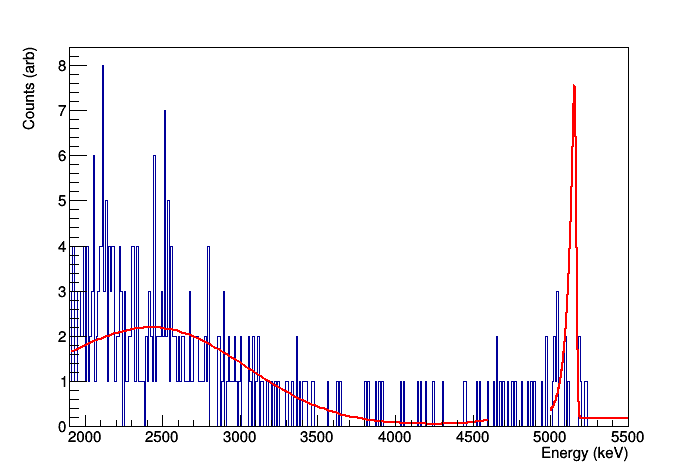
\includegraphics[height=3in]{/Users/jgruszko/Documents/Thesis/Plots/Ch6/MJ_fit_wCorrectFunc_TUBEpk.png}
 \caption{The fit result with an unmodified point-contact even peak shape.}
 \label{fig:r2spec_orig}
  \end{subfigure}
 \begin{subfigure}[]{\textwidth}
 \centering
 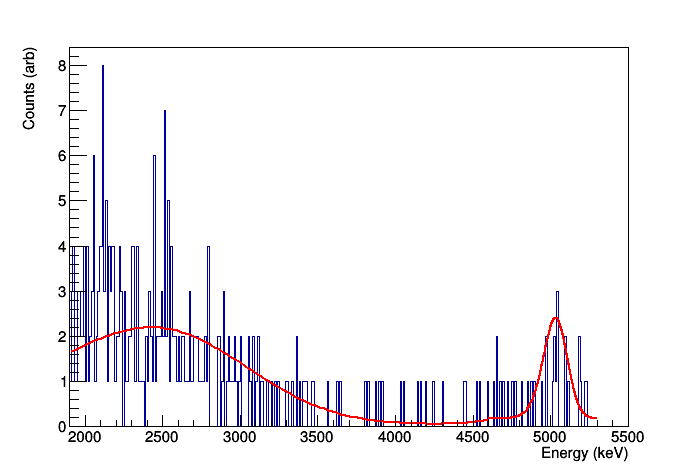
\includegraphics[height=3in]{/Users/jgruszko/Documents/Thesis/Plots/Ch6/MJ_fit_wCorrectFunc_mu5064sig70pk.png}
  \caption{The same passivated-surface spectrum fit result with the width and centroid of the point-contact event peak shape adjusted to approximate the observed shape.}
 \label{fig:r2spec_mod}
 \end{subfigure}
 \caption[A fit of the point contact contamination model to the \MJ\ \DEM\ energy spectrum]{The high-energy spectrum from the \MJ\ \DEM\, data sets 0-5, with muon, data cleaning, single-site, and multiplicity cuts applied, in blue. The point-contact contamination model for passivated surface events (in red) was fit to the data, and the predicted scaling was applied to the point-contact peak shape model.} 
 \label{fig:mjSpec_fit}
\end{figure}


